\documentclass[12pt]{article}
\usepackage[utf8]{inputenc}
\usepackage{graphicx}
\usepackage{float}
\usepackage{packages}

\begin{document}

\import{./}{title}

\import{./}{declaration}

\frontmatter

\tableofcontents

\mainmatter

\section{Introduction}
\label{section: intro}
Team Two's project is a load balancer simulation system. Load balancers are widely used to reduce excessive resource consumption across servers when serving high volume traffic. This project is a simulation system with some simplifying assumptions regarding load balancer. The assumptions are as follows:

\begin{enumerate}
    \item The system is running in a secure environment. In production, a real load balancer is run in a secure environment such as kubernetes where rule sets and firewalls have been configured. This means that it is currently devoid of any encryption under this assumption
    \item  Internet protocol generation and management is trivial in this system. It assumes an internet protocol address is simply a pointer to a file on the system. An example of an internet protocol address in system could be "ip1.txt". The system would then call relative modules to write requests to this file which is considered as the internet protocol address has been successfully reached.
    \item Any requests are the simplified HTTP requests in this system. It does not faithfully adhere to HTTP protocol in format.
\end{enumerate}

\section{Use Cases and Requirements}
\label{section: use_case_and_requirements}
The project requirements and use case diagrams are as follows. It follows the \textbf{SMART} principle: \textbf{S} - Specific \textbf{M} - Measurable \textbf{A} - Attainable \textbf{R} - Realisable \textbf{T} - Traceable

The list of functional requirements is also outlined below 
% All requirements should be SMART. Be reasonably general whilst still being relevant
% If a few requirements can be wrote as a single requirement then that is preferred as we don't need pages of requirements 
%\begin{enumerate}
    %\item \textbf{Reliability} Route requests to the correct server. This will be measured and traced via a correct write to the internet protocol address which, in the context of this simulation, will be a pointer to a file on the system.
   % \item \textbf{Performance} The simulation should be performant when dealing with client requests. This will be measured and traced via unit testing and logging.
%\end{enumerate}
% As per feedback I think a small number of functional requirements that encompass everything is better than a bunch of smaller ones 
\begin{enumerate}
    % text Log files is something the reader will understand as its a general term
    \item The system must allow a client to send a request and can be measured and traced via text log files.
    % The reader is on page 1. They have no idea what our system does. We have to assume no knowledge and explain it to them in an understandable way.What is server list? The reader will not understand 
    \item The system must contain a pool to store all servers and allow new servers to be added. A pool is defined as a grouping of valid of servers. A valid server, in the context of this project, is a server that has done the following: \textbf{A} assigned itself an internet protocol address \textbf{B} added itself to the server pool. More information can be found in section \ref{section: implementation}.
    %Again what is algorithms? Are we talking resource based algorithms? What specific algorithms are we using? Define different user requests? What requests can the user make in our system? The person reading this document is only on page 1. They will not understand what you are talking about
    \item The system should handle client requests and distribute client requests to the appropriate server(s).
    %What algorithms? What is the transmit tool? They are only on page 1. Assume they have never seen the code. Again the user has no understanding of our system
    %\item The system should determine a target server by algorithms after the user's request reach the load balancer, the transmit tool should pass the user's request to this server.
    % What is listening? What are we listening for? The reader will not have an proper understanding of our system so it needs to be easily understandable by anyone 
    \item The system should start listening and is ready to transmit resources once the client request reaches a specific server. The listening concept in this project is a valid server that is ready to receive client requests. 
\end{enumerate}

The list of non-functional requirements is outlined below 
\begin{enumerate}
    \item \textbf{Testability:} Greater than 80\% test coverage. The reason for choosing 80\% is it covers critical aspects of the code whilst keeping the tests relevant. Aiming for 90\% or above can mean that tests often end up being written to achieve the test coverage target and do not add value.
    \item \textbf{Logging:} Log requests that are sent through the simulation to a text file for transparency and diagnostics. 
    
    %I don't think these are SMART, how will we test this? Ensure its traceable?
    % Do we have unit tests written for this? We can add this for the final deliverable once we can prove its traceable and testable
    %\item\textbf{Testability}: The project applies the JUnit 5 testing framework, the test coverage should be 80\%, thus it cover critical aspects of the code whilst keeping the tests relevant.
    \item\textbf{Performance}: After applying the load balancing algorithm, the processing time of user requests can be reduced by 70\% in the face of the same number of users accessing at the same time.
    \item\textbf{Capacity}: The project expects that the load balancer can handle the requests of up to 50 users at the same time.
    \item\textbf{Availability}: The load balancer should provide 99\% availability, also known as a service level agreement.
\end{enumerate}
\subsection{Use Case Diagram and Sequence Diagram}
The use case diagram and sequence diagram are as follows. 

% This is the load balancer sequence diagram 
\begin{figure}[H]
    \centering
    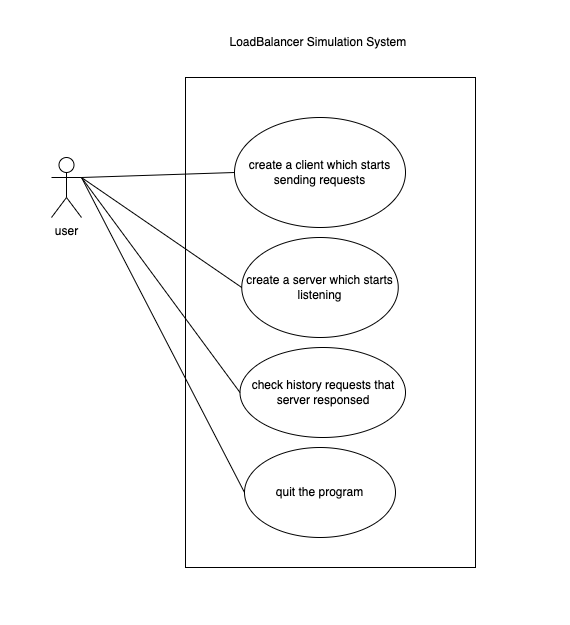
\includegraphics[width=\linewidth]{images/uc.png}
    \caption{Use Case Diagram}
    \label{fig:Use_Case_Diagram}
\end{figure}

% This is the server pool sequence diagram 
\begin{figure}[H]
    \centering
    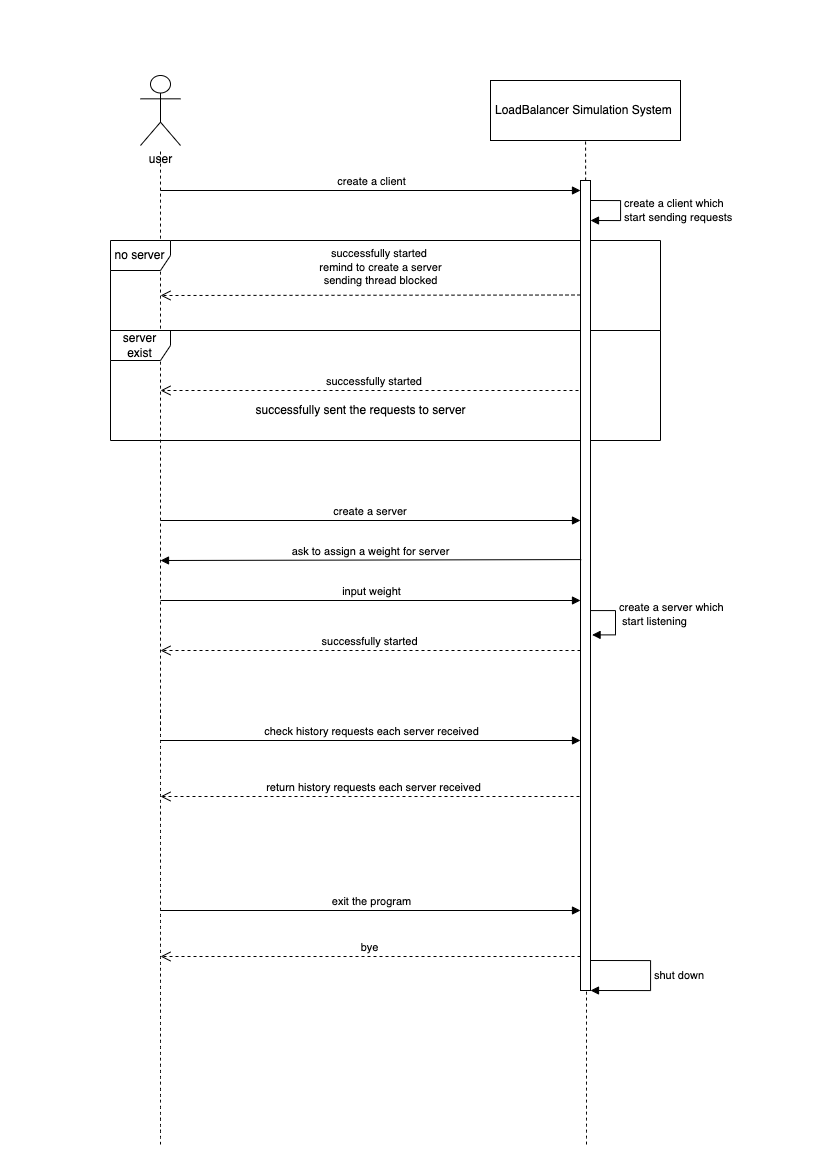
\includegraphics[width=\linewidth]{images/seq.png}
    \caption{Sequence Diagram}
    \label{fig:Sequence_Diagram}
\end{figure}

The use case diagram and sequence diagram show the basic functions of this system. 

Users can add a client or a server in this simulation system. If the user adds a client, the system will call the Client module to start a client thread which starts sending simulated requests to the server. If at least one server exists, the requests will be dispatched by the load balancer module in the system and finally be written into different simulated servers( server files under server folder ). Otherwise, the client thread will be blocked for the time being and reminds user to create a new server every 10 seconds.

If the user adds a server, the system will call the Server module to create a server file under the server folder and register the server to the server pool. The load balancer will refresh the list of server from server pool every time the pool updates.

The requests are dispatched by the load balancer module which calls the Algorithm module to pair a server for each request. 
Once a request is assigned to a server, the system will create a socket to store the request and server ip information. After all requests have been assigned, the system will pass the list of sockets to the Transmit Tool module to start transmissions between clients and servers.

Users can exit the system if they want.

\subsection{Finite State Machine and Data Flow Diagram}

\begin{figure}[H]
\centering
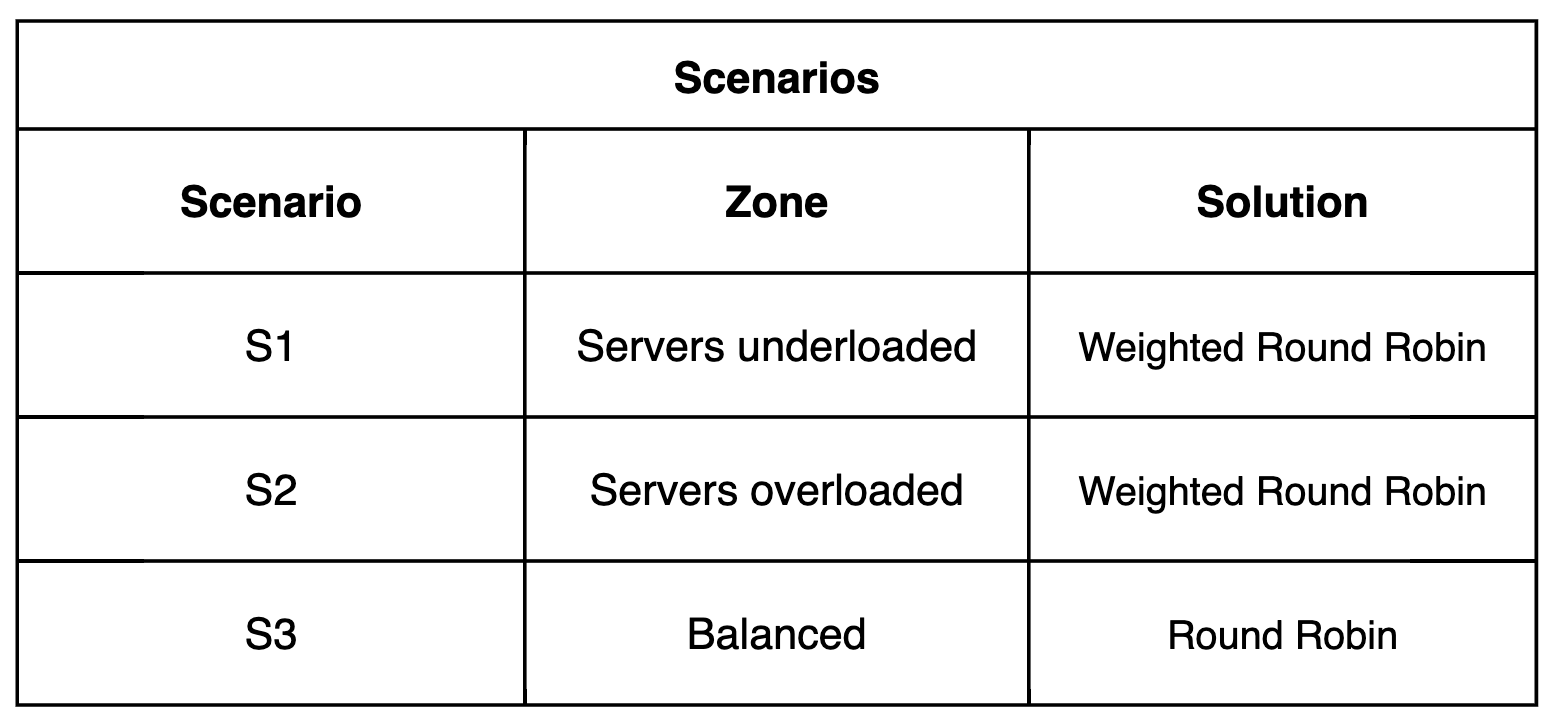
\includegraphics[width=\linewidth]{images/load_balancer_scenarios.jpg}
\caption{Finite State Machine - Scenarios}
\label{fig:Scenarios}
\end{figure}

The scenarios table in Figure \ref{fig:Scenarios} is the list of the possible scenarios based on the server’s load. Depending on the load of the servers, a solution will be given for each scenario. In S1, the servers are underloaded so the weighted round robin algorithm will be used. The same will apply for S2 when the servers are overloaded. For S3, when the load is balanced, that’s when round robin will be used instead of the weighted round robin algorithm.

\begin{figure}[H]
\centering
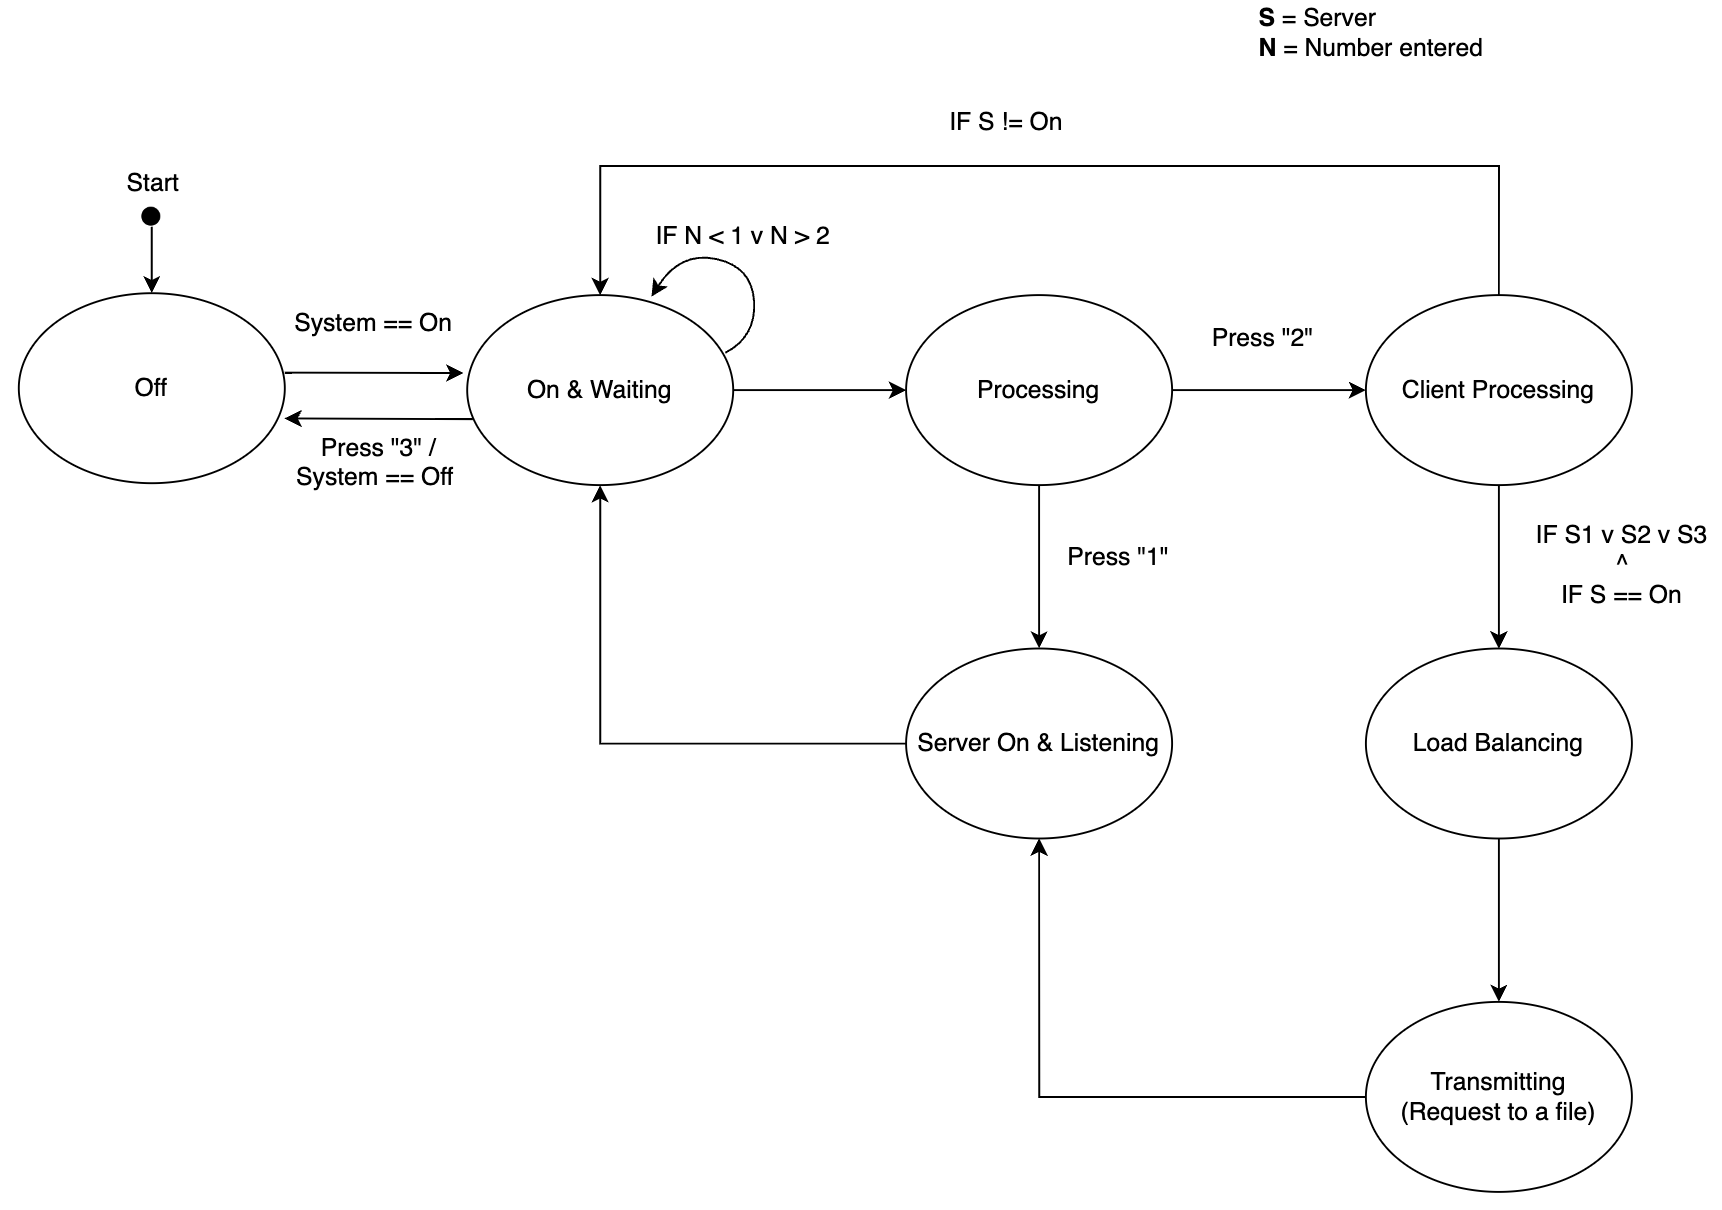
\includegraphics[width=\linewidth]{images/load_balancer_finite_state_machine.jpg}
\caption{Finite State Machine}
\label{fig:Finite_State_Machine}
\end{figure}

Figure \ref{fig:Finite_State_Machine} is a diagram of our finite state machine of the load balancer system. The system starts off in the “Off” state. When the system is powered on, it will be waiting for user input. If “3” is entered then the system will turn off. While in the “On and Waiting” state, if the number entered is less and 1 or greater than 2 then the system will remain in its current state. Let’s say “1” has been pressed. The user can enter the weight of the server, the server will then be initialised and the server module will register itself to the pool of servers. It remains in the “Server On and Listening” state until the user turns off the system. Suppose the server is on and the user has entered “2”. The client module is now in a “processing” state meaning that it will begin to send requests to the server. The requests will be sent to the load balancer, the load balancer retrieves the server pool and an algorithm will be selected according to the server’s current load. This is accomplished in the “Load Balancing” state. In the “Transmitting” state, the requests will be received by the transmit tool and it will simply write a message to the server. 

\begin{figure}[H]
\centering
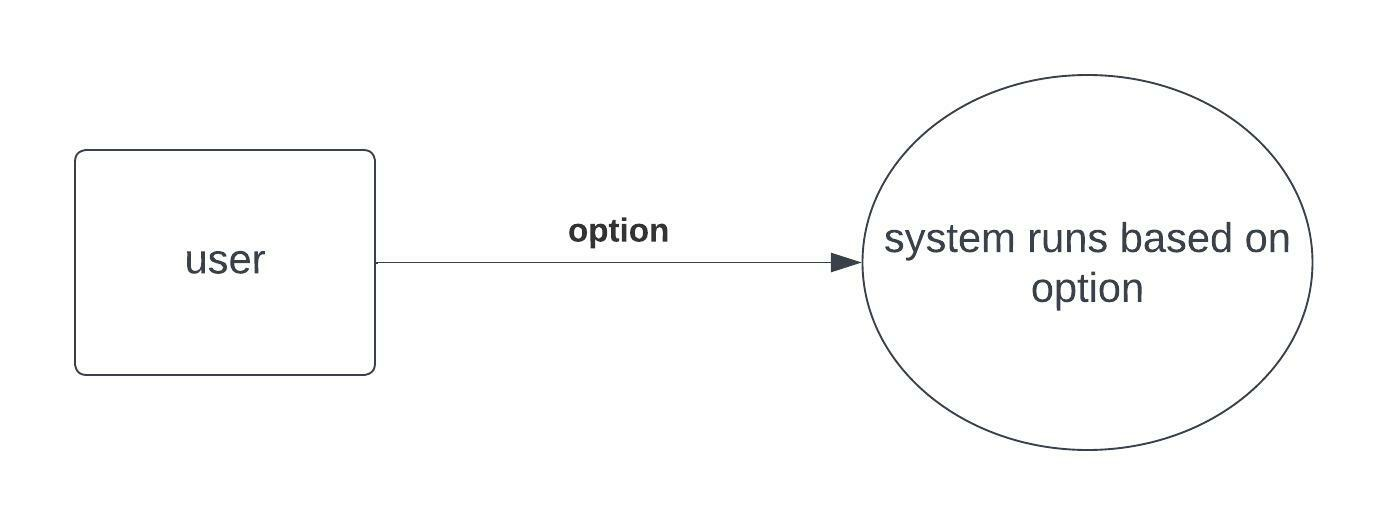
\includegraphics[width=\linewidth]{images/context_diagram.jpeg}
\caption{Context Diagram}
\label{fig:context_diagram}
\end{figure}
The above context diagram shows that the load balancer system takes the user option and starts running based on the option. More details will be discussed in the first-level dataflow diagram.

\begin{figure}[H]
\centering
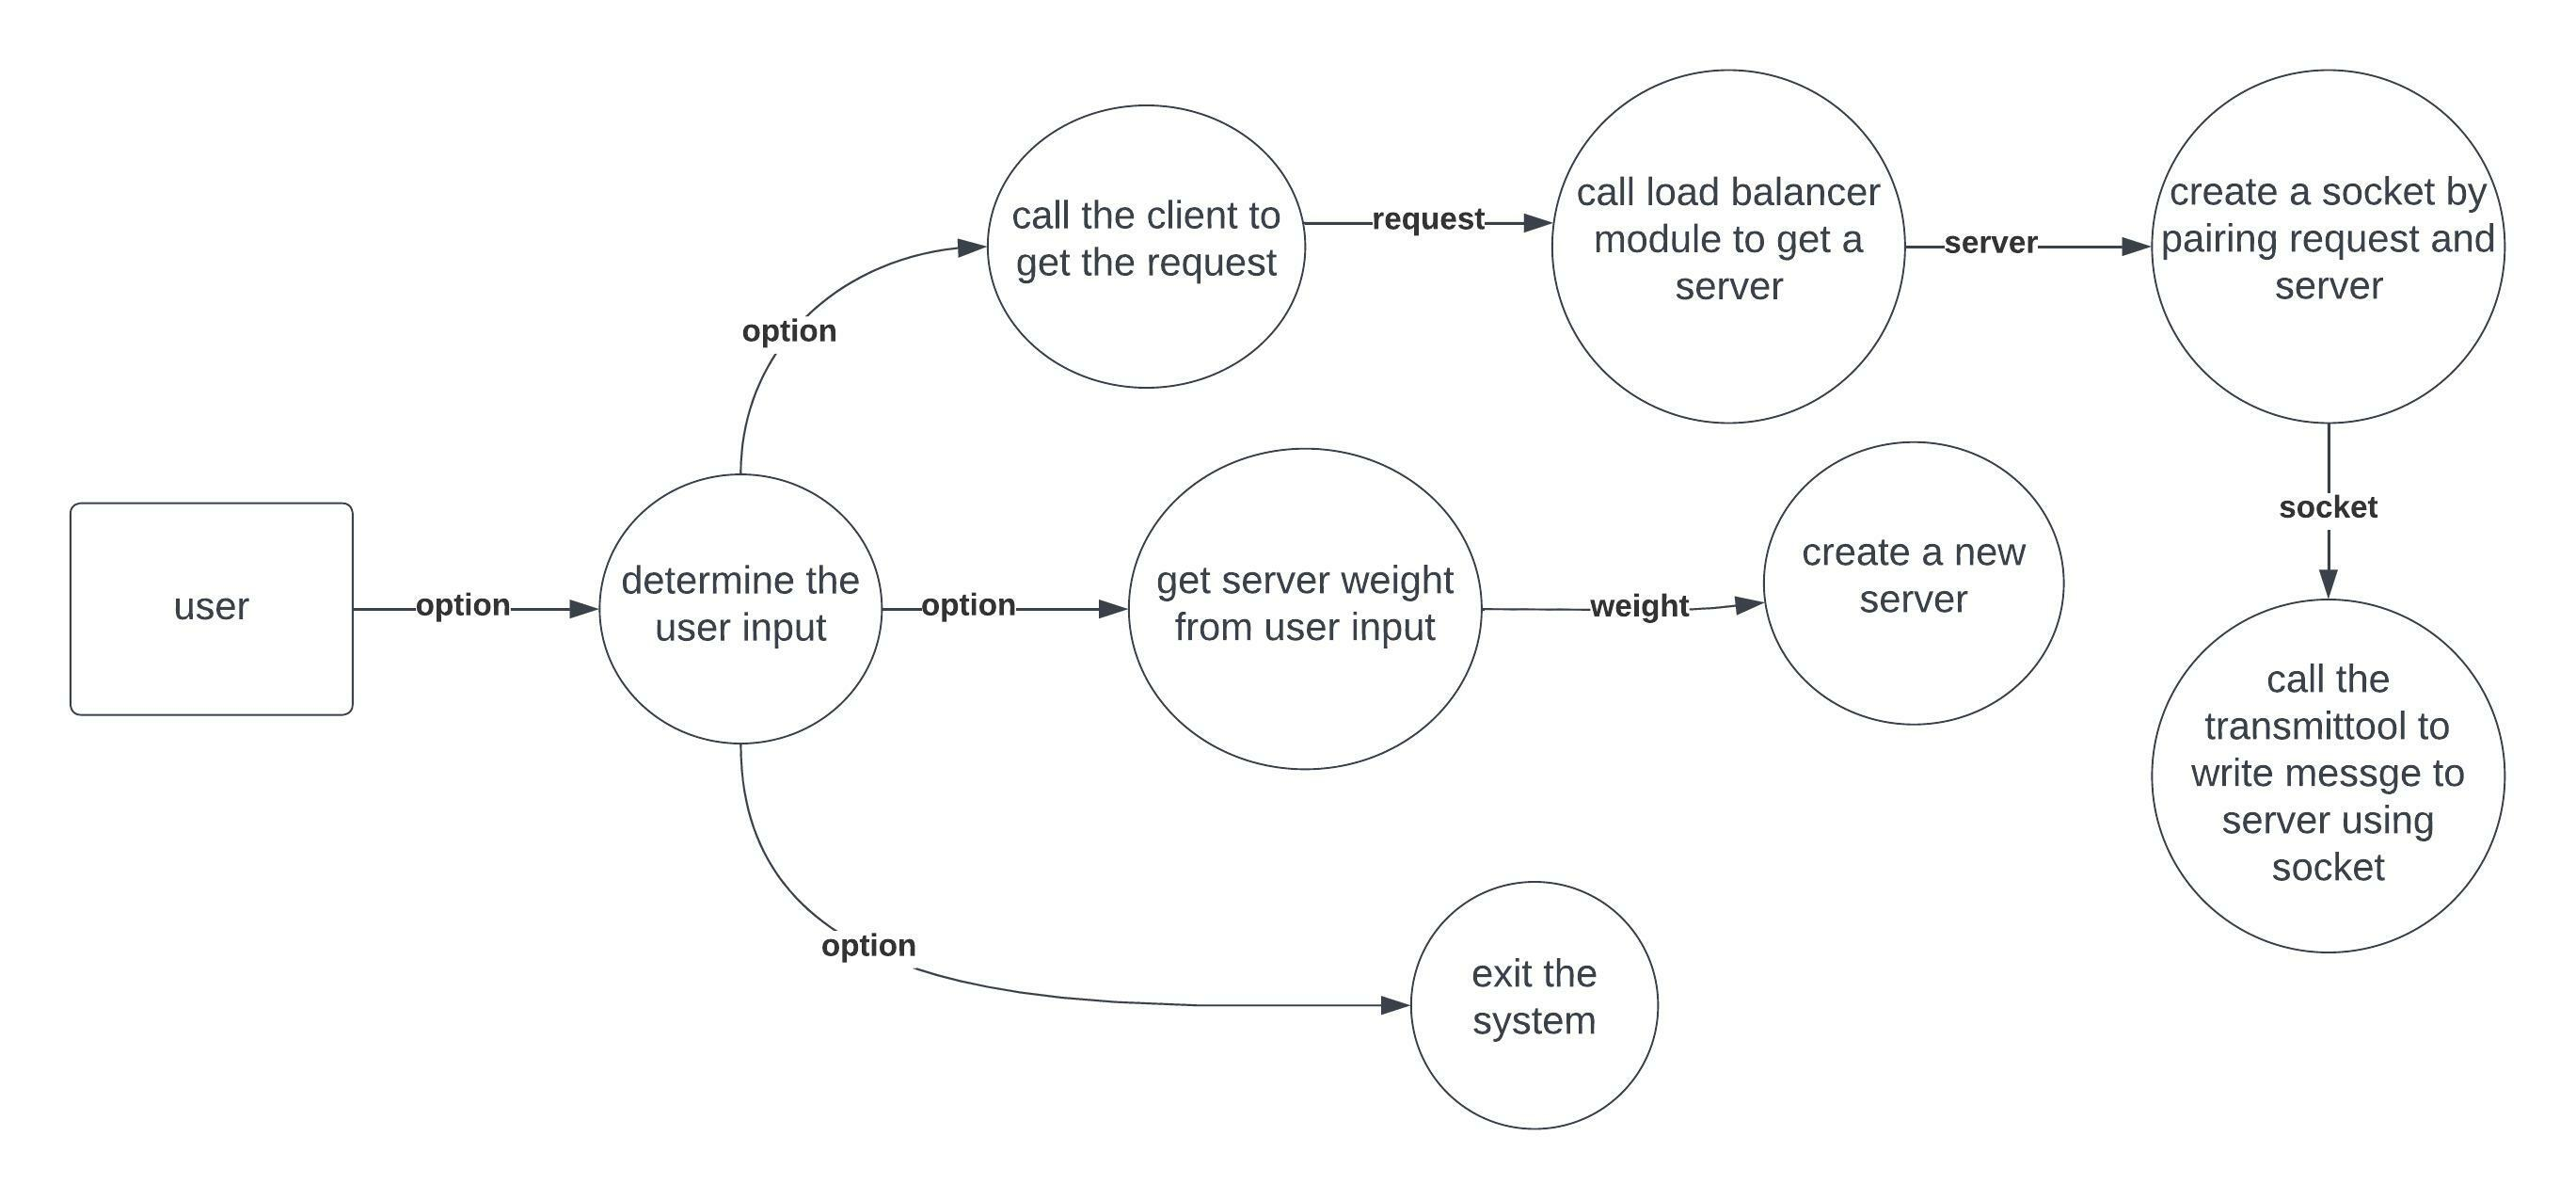
\includegraphics[width=\linewidth]{images/dataflow_diagram.jpeg}
\caption{Dataflow Diagram}
\label{fig:Data_flow_diagram}
\end{figure}
There are three scenarios in total based on the user's input:
\begin{enumerate}
\item Create a server.
If a user sends a request, the system will call the client to get the request. The Load balancer then gets the list of servers from the server pool and uses load balancing algorithm to choose a server. Then the system creates a socket by pairing the server with the request and sends the socket to the transmit tool. The Transmit tool writes a message to the server by using the socket. 
\item Send a request.
If the user wants to create a server, the system will ask the user to assign a weight to the server which indicates the capacity of the server. Then a new server will be created and starts listening.
\item Exit the system.
If the user chooses to exit the system, the system will stop.
\end{enumerate}

\section{Design and Analysis}
\label{section: design_and_analysis}
This section mainly discusses and analyses the design. It refers to use case diagrams and code snippets where appropriate. Any referred code snippets are taken from the project code. For implementation details please see section \ref{section: implementation}.

As stated in the introduction, this system is a simulation of a load balancer. It was designed in loosely coupled, modular fashion for easy changes that may occur in the future. The diagram below shows the system at a high level.

\begin{figure}[H]
    \centering
    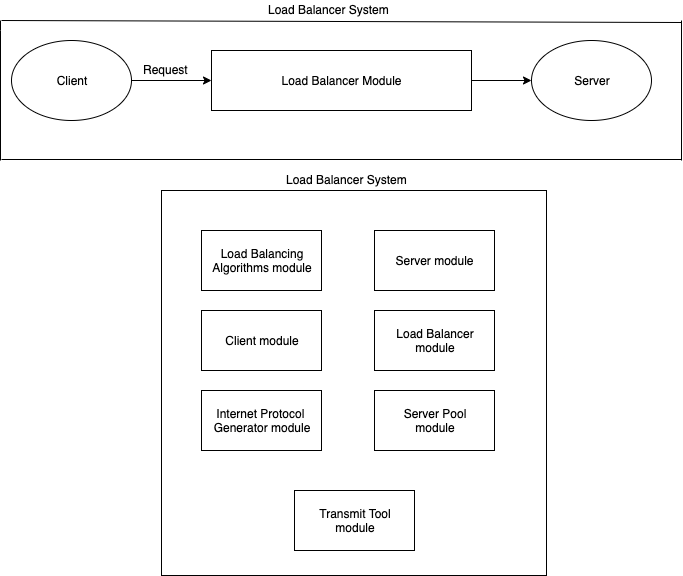
\includegraphics[width=\linewidth]{images/System_Overview.png}
    \caption{System Design Overview }
    \label{fig:System_overview}
\end{figure}

At the most basic level the client submits a request for a server. As stated in section \ref{section: intro} simplifying assumptions has been made about the client request. The load balancer system takes this request and forwards it to the appropriate server.  This simple system overview diagram shows the critical relationships among client module, loadbalancer module, and server module. The load balancer system's job is to dispense requests from clients to the servers through the loadbalancer module.

The box under the load balancer system shows the different modules at work to help the simulator achieve its objectives. These modules are described in detail in section \ref{section: implementation}. By opting for this modular approach and delegating tasks to different modules, it means our system design is more prepared for change, if and when that may occur. An example is by separating the load balancing algorithms module, which contains implementations of Round-robin and Weighted Round-robin, from the load balancer module, we enable easy addition and deletion of load balancing algorithms. The load balancer module essentially delegates its tasks to the different modules for maximum flexibility for change down the line. Now that approaches to the overall design of the system have been discussed, the following topic will discuss reasons for choosing Round-robin and Weighted Round-robin algorithms for the load balancer. They are both similar but there are some important distinctions between them.

\subsection{Round-Robin}
Round Robin is a type of scheduling algorithm\cite{RR}. Scheduling algorithms aim to optimally schedule events so as to minimise something, that something could include minimising CPU wastage, in the case of operating systems. In the case of load balancers scheduling algorithms seek to optimally schedule requests to minimise wait time and resource usage amongst a group of servers, also known as a server pool. Round Robin works by dividing up incoming requests equally, and distributing them amongst the server pool. Round robin is starvation free. This avoids the issue of resource starvation, whereby a request is perpetually denied due to unavailability of the necessary resources to process the request. 


\subsection{Weighted Round Robin}
Weighted Round Robin is another type of scheduling algorithm\cite{WRR}. The main difference between Weighted Round Robin and Round Robin is the addition of weights. Not all servers are created equally, some can handle more requests than others. Therefore it makes sense to assign a higher weight to a more powerful server and a lower weight to a less powerful server. Essentially this means that more powerful servers will be assigned more requests and less powerful servers will be assigned less requests. This has the effect of being much more realistic in terms of real world scenario's whereby the servers might be of different configurations, different memory allocations and CPU allocations, and it is necessary to take this into account to operate optimally. Like Round-Robin, it is also starvation free. 

\section{Implementation}
\label{section: implementation}
Please see our demo\cite{Video}
This section will describe in detail the implementation details, including snippets of code where necessary. Please see \cite{repo} - The project is implemented in the Java programming language. Java is an ideal choice as it is heavily documented with many online resources available and highly follows object-oriented principles. Conscious design choices have been made to achieve flexibility, scalability, and reliability. The outline  structure of this project shows below. This project is mainly composed of eight classes. 
\begin{itemize}
    \item Runner.java
    \item Algorithm.java
    \item IpGenerator.java
    \item LoadBalancer.java
    \item Server.java
    \item ServerPool.java
    \item TransmitTool.java
    \item Client.java
\end{itemize}

We now give a brief overview of the purpose of each class, and how each class fits into the overall project.

\subsection{Class Details}
\begin{enumerate}
    \item \textbf{Runner.java: }This is the class that hosts the main method. Essentially this is the entry point and runner for the project 
   \item \textbf{Algorithm.java: }This is the class that hosts the scheduling algorithm(s). We have included the option of two known scheduling algorithms, Round Robin and Weighted Round Robin. By separating the algorithm from the implementation we allow for greater flexibility for changes that may occur in the future.
   \item \textbf{IpGenerator.java: }This is the class that is responsible for assigning internet protocol addresses to each of the servers. As we are simulating a load balancer, we have elected to have the internet protocol address be a pointer to a file on the system. An example of an internet protocol address within the context of this project would be 'IP1.txt'. We can then verify the client accessed the resource they requested by writing to this file. The files are not hard coded, instead they are created at run time.
   \item \textbf{LoadBalancer.java: }This is the class that provides an available server for a request by using Algorithm module and ServerPool module each time call. It gets the list of server info from ServerPool and call the Algorithm module to pick a server from the list. After the load balancer returns the server, system will create a socket for the request and the server and add it to a list.
   \item \textbf{Server.java: }This is the class that describes the server. It includes some methods that the server will need in order to be a valid server. We define a valid server, in the context of this project, as being a server that has done the following: \textbf{A} assigned itself an internet protocol address \textbf{B} added itself to the server pool. 
   \item \textbf{ServerPool.java: }This is the class that describes the server pool. We define a server pool in the context of this project as a grouping of valid servers. There is no limit on the number of valid servers that can be in the server pool. We keep track of the valid servers in the server pool via an array list. Each time a valid server is created we add it to the array list.
   \item \textbf{TransmitTool.java: }This class is responsible for connection and transmission between client and server. It stores list of Socket class objects. A Socket class object stores one pair of client and server ip address along with request messages. After main thread created a list of sockets by using Load balancer module, system will set the list of sockets into TransmitTool and call the send method of it to start transmitting. TransmitTool will write request messages into servers by using sockets. After transmission, it will clear and refresh the list of sockets inside. 
   \item \textbf{Client.java: }This is the class that is responsible for receiving client requests via a text file. Every line is read in from the file and the information will then be sent to the LoadBalancer class.
\end{enumerate}

\section{Tests}
In addition to the eight classes, we also have corresponding test classes. We used Junit5 to implement the unit tests. We outline these test classes 
\begin{itemize}
    \item AlgorithmTest.java
    \item IpGeneratorTest.java
    \item LoadBalancerTest.java
    \item ServerTest.java
    \item ServerPoolTest.java
    \item TransmitToolTest.java
    \item ClientTest.java
\end{itemize}

We based our testing philosophy around testing important functionality rather than writing tests to achieve an arbitrary test coverage statistic. We now give an overview of the purpose of each class and what important functionality we are testing.

\subsection{Class Details}
\begin{itemize}
    \item \textbf{AlgorithmTest: }We aim to test critical aspects of the Round Robin and Weighted Round Robin algorithm(s). We test that it correctly sets the weight, that it correctly selects the next server in the case of Weighted Round Robin or in the case of Round Robin, just that it selects the correct server as there is no weight used. 
    \item \textbf{IpGeneratorTest: }We aim to test critical aspects of the internet protocol generator. Namely we aim to test that the simulated internet protocol is assigned correctly. 
    \item \textbf{LoadBalancerTest: }We aim to test the load balancer can continuously return a server by using Algorithm and ServerPool module given a specified value of call time. We expect the sequence of severlist that the load balancer returns is same with the specified one.
    \item \textbf{ServerTest.java: }We aim to test critical aspects of the Server. We aim to test that the server is a valid server.This involves testing that the internet protocol address can be retrieved successfully and that it is the correct internet protocol address. It also involves testing the server can add itself to the server pool 
    \item \textbf{ServerPoolTest.java: }We aim to test that critical aspects of the server pool are working properly. This involves testing the getters and setters of the server pool and that we can successfully add servers to the server pool and that all values are what we expect them to be 
    \item \textbf{TransmitToolTest.java: }We aim to test that TransmitTool can successfully write request messages into servers by using list of sockets. This involves simulating a list sockets and servers, calling the send method of TransmitTool and get expected list of requests in each server file.
    \item \textbf{ClientTest.java: } We aim to test the readFile method to ensure that we are reading in the file properly and comparing the lines in the file to a string of data.
    
\end{itemize}
\section{References}
\printbibliography[heading=none]
\end{document}